\section{简并半导体}
在过去几节中,我们对于载流子浓度的计算都是基于\fancyref{fml:导带电子浓度}
\begin{Equation}
    n_0=N_\text{c}\exp(\frac{E_\text{F}-E_\text{c}}{\kB T})
\end{Equation}
但是,该公式的推导的前提条件是$E_\text{c}-E_\text{F}\gg \kB T$,换言之,导带底距离费米能级应有一定的距离,以确保导带的电子分布可以适用玻尔兹曼分布。然而,这个条件并不是总能满足的。

根据\fancyref{fml:高温强电离区的费米能级}
\begin{Equation}
    E_\text{F}=E_\text{c}+\kB T\ln\qty(\frac{N_\text{D}}{N_\text{c}})
\end{Equation}
\begin{itemize}
    \item 当掺杂浓度$N_\text{D}<N_\text{c}$时,对数项为负,此时$E_\text{F}<E_\text{c}$,导带可适用玻尔兹曼分布。
    \item 当掺杂浓度$N_\text{D}>N_\text{c}$时,对数项为正,此时$E_\text{F}>E_\text{c}$,导带应适用费米分布。
\end{itemize}
由此可见,如果掺杂浓度很高,就会使得费米能级从禁带上移至导带,使我们在讨论导带电子浓度时,不再能使用近似的玻尔兹曼分布,必须要用费米分布,换言之,材料由非简并半导体转化为了简并半导体。在本节,我们将在费米分布的背景下,重新推演适用于简并半导体的载流子浓度公式(相当于\xref{sec:载流子浓度}的工作),探讨简并的发生条件,研究简并半导体的掺杂性质。

\subsection{简并半导体的载流子浓度}
我们先以简并半导体的电子浓度为例讨论,很显然,电子浓度可以表示为\setpeq{简并半导体的载流子浓度}
\begin{Equation}&[1]
    n_0=\frac{1}{V}\Int[E_\text{c}][E_\text{c}']f(E)g(E)\dd{E}
\end{Equation}
简并半导体与非简并半导体的根本差异在于,后者的$f(E)$为玻尔兹曼分布,前者的$f(E)$为费米分布。因此,原先非简并半导体情形下的推导中的\xrefpeq[导带电子浓度]{4}在这里就应当改为
\begin{Equation}&[2]
    n_0=\frac{1}{2\pi^2}\frac{(2\mne)^{3/2}}{\hbar^3}\exp(\frac{E_\text{F}-E_\text{c}}{\kB T})\Int[E_\text{c}][E_\text{c}']
    \frac{(E-E_\text{c})^{1/2}}{1+\exp(E-E_\text{F}/\kB T)}\dd{E}
\end{Equation}
和过去一样,我们引入$N_\text{c}$和$x$作代换,这里还要引入$\xi$
\begin{Equation}&[3]
    N_\text{c}=2\qty(\frac{\mne\kB T}{2\pi\hbar^2})^{3/2}\qquad
    x=\frac{E-E_\text{c}}{\kB T}\qquad
    \xi=\frac{E_\text{F}-E_\text{c}}{\kB T}
\end{Equation}
将\xrefpeq{3}代入\xrefpeq{2}
\begin{Equation}&[4]
    n_0=N_\text{c}\frac{2}{\sqrt{\pi}}\Int[0][x']\frac{x^{1/2}}{1+\e^{x-\xi}}\dx
\end{Equation}
这样问题又回到了积分的计算
\begin{Equation}
    I=\Int[0][x']\frac{x^{1/2}}{1+\e^{x-\xi}}\dx
\end{Equation}
这里将积分上限由$x'$改为$\infty$也不会有太大的误差
\begin{Equation}
    I=\Int[0][\infty]\frac{x^{1/2}}{1+\e^{x-\xi}}\dx
\end{Equation}
然而,相较于非简并半导体中遭遇的高斯积分,这里的积分要复杂的多,而且是含参的。我们将这类积分称为\uwave{费米积分},将其积分结果称为\uwave{费米函数},作为一种特殊函数,定义如下。
\begin{BoxDefinition}[费米函数]
    费米函数被定义为
    \begin{Equation}
        \Ffermi_{1/2}(\xi)=\Int[0][\infty]\frac{x^{1/2}}{1+\e^{x-\xi}}\dx
    \end{Equation}
\end{BoxDefinition}

费米函数的图像,如\xref{fig:费米函数}所示,分别用普通坐标和对数坐标绘制。我们在\xref{fig:费米函数}中注意到,费米函数$\Ffermi_{1/2}(\xi)$的增长趋势在初期大致与线性函数$2\xi$相近(但后期会快些),因此,费米函数在对数坐标下的形态类似对数函数\footnote{线性函数在对数坐标系下,看起来就像是普通坐标下的对数函数。},这很重要,因为费米函数通常都是在对数坐标下被绘制。

费米函数的一个重要性质是其在$\xi=0$处的值\footnote{从\xref{fig:费米函数}中可以看出,这大约是零点几。},有趣的是,这是一个有理数。
\begin{BoxProperty}[费米函数的特殊值]
    费米函数在$\xi=0$处的值为
    \begin{Equation}
        \Ffermi_{1/2}(0)=0.6
    \end{Equation}
\end{BoxProperty}
\begin{Figure}[费米函数]
    \begin{FigureSub}[普通坐标的费米函数]
        \hspace{1.8cm}
        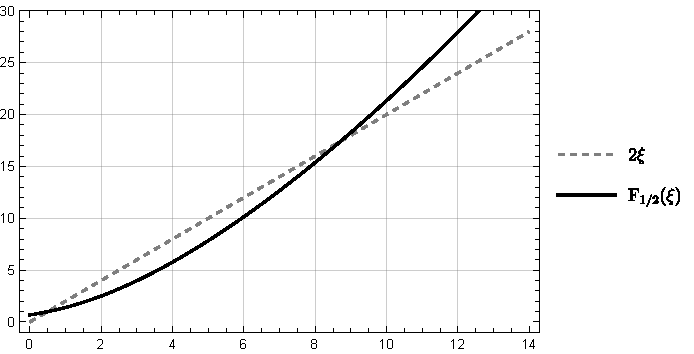
\includegraphics[scale=0.85]{Mathematica/output/FermiFunc.pdf}
    \end{FigureSub}\vspace{0.5cm}
    \begin{FigureSub}[对数坐标的费米函数]
        \hspace{1.8cm}
        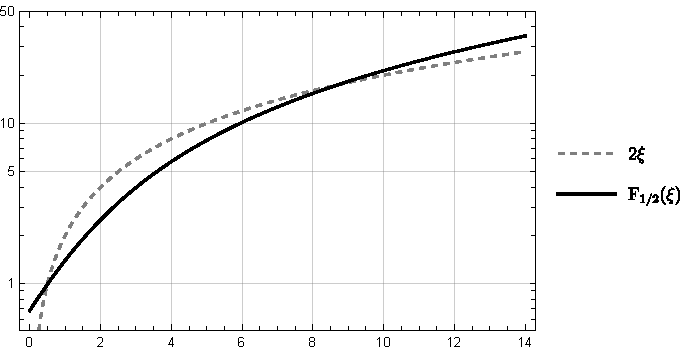
\includegraphics[scale=0.85]{Mathematica/output/FermiFuncLog.pdf}
    \end{FigureSub}
\end{Figure}

引入了费米函数后,\xrefpeq[简并半导体的载流子浓度]{4}就可以表示为
\begin{Equation}
    n_0=N_\text{c}\frac{2}{\sqrt{\pi}}\Ffermi_{1/2}\qty(\xi)=N_\text{c}\frac{2}{\sqrt{\pi}}\Ffermi_{1/2}\qty(\frac{E_\text{F}-E_\text{c}}{\kB T})
\end{Equation}
这样就得到了简并半导体中电子浓度$n_0$的表达式
\begin{BoxFormula}[简并半导体的电子浓度]
    简并半导体中,电子浓度满足
    \begin{Equation}
        n_0=N_\text{c}\frac{2}{\sqrt{\pi}}\Ffermi_{1/2}\qty(\frac{E_\text{F}-E_\text{c}}{\kB T})
    \end{Equation}
\end{BoxFormula}
这里也可以类似得到简并半导体中空穴浓度$p_0$的表达式
\begin{BoxFormula}[简并半导体的空穴浓度]
    简并半导体中,空穴浓度满足
    \begin{Equation}
        p_0=N_\text{v}\frac{2}{\sqrt{\pi}}\Ffermi_{1/2}\qty(\frac{E_\text{v}-E_\text{F}}{\kB T})
    \end{Equation}
\end{BoxFormula}

\subsection{简并化条件}
现在让我们来对比一下非简并半导体和简并半导体中的载流子浓度公式。

根据\xref{fml:导带电子浓度},非简并半导体中的载流子浓度为
\begin{Equation}
    n_0=N_\text{c}\exp(\frac{E_\text{F}-E_\text{c}}{\kB T})
\end{Equation}
根据\xref{fml:简并半导体的电子浓度},简并半导体中的载流子浓度为
\begin{Equation}
    n_0=N_\text{c}\frac{\sqrt{\pi}}{2}\Ffermi_{1/2}\qty(\frac{E_\text{F}-E_\text{c}}{\kB T})
\end{Equation}
由此可见,简并半导体和非简并半导体的载流子浓度公式是相近的,我们可以绘图对比。
\begin{Figure}[载流子浓度曲线]
    \begin{FigureSub}[普通坐标的载流子浓度曲线]
        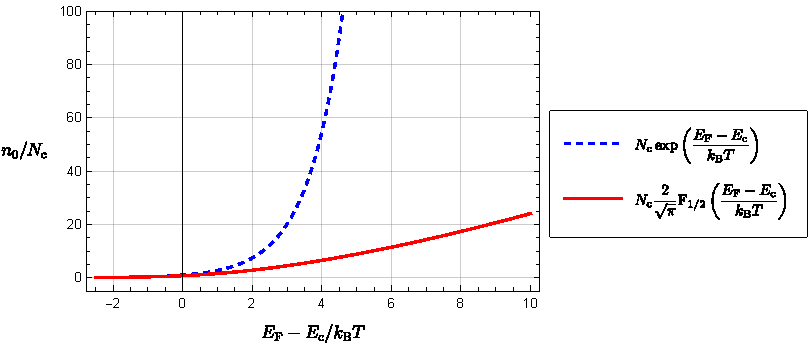
\includegraphics[scale=0.9]{Mathematica/output/Degenerate.pdf}
    \end{FigureSub}\vspace{0.5cm}
    \begin{FigureSub}[对数坐标的载流子浓度曲线]
        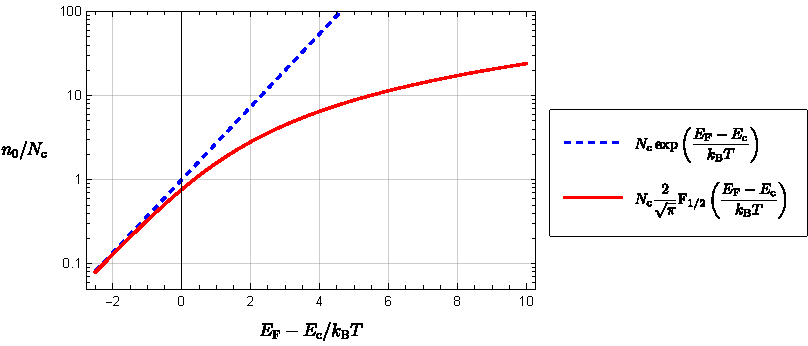
\includegraphics[scale=0.9]{Mathematica/output/DegenerateLog.pdf}
    \end{FigureSub}
\end{Figure}
由\xref{fig:载流子浓度曲线}可以看出,简并化与否,关键在于$E_\text{F}-E_\text{c}/\kB T$的取值
\begin{itemize}
    \item 定义\uwave{非简并},指满足$E_\text{F}-E_\text{c}/\kB T<-2$的情形。
    \item 定义\uwave{弱简并},指满足$E_\text{F}-E_\text{c}/\kB T>-2$且$E_\text{F}-E_\text{c}/\kB T<0$的情形。
    \item 定义\uwave{简并},指满足$E_\text{F}-E_\text{c}/\kB T>0$的情形。
\end{itemize}
现在,我们用$E_\text{F}$和$E_\text{c}$的关系定义了简并化和非简并化的标准,因此,如果我们要研究半导体何时会发生简并,就是要研究$E_\text{F}=E_\text{c}$时(这里认为弱简并不算简并)杂质浓度$N_\text{D}$的阈值取值,换言之,若掺入的杂质浓度达到了相应的阈值,就有$E_\text{F}=E_\text{c}$成立,材料简并化。

我们运用\fancyref{fml:高温强电离区的电中性条件},这也适用于简并半导体(N型)
\begin{Equation}
    n_0=n_\text{D}^{+}
\end{Equation}
代入\fancyref{fml:简并半导体的电子浓度}和\fancyref{fml:施主浓度}
\begin{Equation}
    N_\text{c}\frac{2}{\sqrt{\pi}}\Ffermi_{1/2}\qty(\frac{E_\text{F}-E_\text{c}}{\kB T})=\frac{N_\text{D}}{1+g_\text{D}\exp(E_\text{F}-E_\text{D}/\kB T)}
\end{Equation}
整理一下
\begin{Equation}
    N_\text{D}=\frac{2N_\text{c}}{\sqrt{\pi}}\qty[1+g_\text{D}\exp(\frac{E_\text{F}-E_\text{D}}{\kB T})]\Ffermi_{1/2}\qty(\frac{E_\text{F}-E_\text{c}}{\kB T})
\end{Equation}
再做些调整,引入$\delt{E}_\text{D}=E_\text{c}-E_\text{D}$
\begin{Equation}
    \qquad\qquad
    N_\text{D}=\frac{2N_\text{c}}{\sqrt{\pi}}\qty[1+g_\text{D}\exp(\frac{E_\text{F}-E_\text{c}}{\kB T})\exp(\frac{\delt{E_\text{D}}}{\kB T})]\Ffermi_{1/2}\qty(\frac{E_\text{F}-E_\text{c}}{\kB T})
    \qquad\qquad
\end{Equation}
在上式中取$E_\text{F}=E_\text{c}$,我们就可以得到发生简并时的杂质浓度。
\begin{BoxFormula}[简并化时的杂质浓度]
    当杂质浓度超过以下阈值后,半导体将简并化
    \begin{Equation}&[A]
        N_\text{D}=\frac{2\Ffermi_{1/2}(0)}{\sqrt{\pi}}\qty[1+g_\text{D}\exp(\frac{\delt{E_\text{D}}}{\kB T})]N_\text{c}
    \end{Equation}
    亦可以将$N_\text
    {c}$代入
    \begin{Equation}&[B]
        \qquad\qquad
        N_\text{D}=\frac{4\Ffermi_{1/2}(0)}{\sqrt{\pi}}\qty(\frac{m_0\kB}{2\pi\hbar^2})^{3/2}\qty(\frac{\mne}{m_0})^{3/2}T^{3/2}\qty[1+g_\text{D}\exp(\frac{\delt{E_\text{D}}}{\kB T})]
        \qquad\qquad
    \end{Equation}
\end{BoxFormula}

通过\xref{fml:简并化时的杂质浓度}可以看出
\begin{itemize}
    \item 函数$\exp(1/T)$是一个随着$T$增大由无穷大逐渐趋近$1$的函数,因此\xrefpeq{A}的方括号的最小值是$3$(简并因子取$g_\text{D}=2$),而根据\fancyref{ppt:费米函数的特殊值},此处的系数$2\Ffermi_{1/2}(0)/\sqrt{\pi}=0.68$,这表明简并化的下限是$N_\text{D}=2.04N_\text{c}$,换言之,如果$N_\text{D}<N_\text{c}$则半导体必然是非简并的。这就定量的论证了掺杂浓度较低时半导体一定是非简并的。
    \item 杂质的电离能$\delt{E_\text{D}}$越宽,在一定温度下,发生简并化时的杂质浓度$N_\text{D}$就越大。
    \item 杂质的电离能$\delt{E_\text{D}}$越窄,在一定温度下,发生简并化时的杂质浓度$N_\text{D}$就越小。
\end{itemize}

通过对\xrefpeq{B}作图可以看出,简并化发生时的杂质浓度$N_\text{D}$与温度的关系,是一个先减小后增大的过程。这就表明,对于某一个杂质浓度(除非其低于$N_\text{D}(T)$的最小值),它将对应一个温度区间,在这个温度区间内半导体会是简并化的。很明显,杂质浓度$N_\text{D}$越高发生简并化的温度区间越宽,并且,杂质浓度$N_\text{D}$一定时,杂质电离能$\delt{E}_\text{D}$越小简并化的温度区间越宽。
\begin{Figure}[简并化时的杂质浓度随温度的变化关系]
    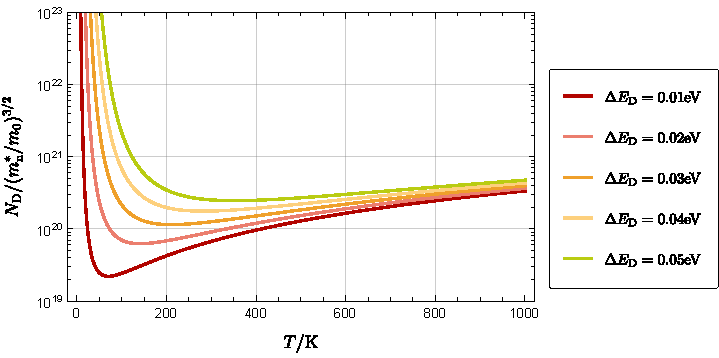
\includegraphics[scale=0.95]{Mathematica/output/DegenerateCT.pdf}
\end{Figure}

对于掺磷的N型锗,磷在锗中的电离能$\delt{E}_\text{D}=0.012\si{eV}$,而据\xref{tab:半导体的状态密度有效质量}锗的$\mne=0.56m_0$,故
\begin{Equation}
    N_\text{D}=3.0\times 10^{19}\si{cm^{-3}}
\end{Equation}
对于掺磷的N型硅,磷在硅中的电离能$\delt{E}_\text{D}=0.044\si{eV}$,而据\xref{tab:半导体的状态密度有效质量}硅的$\mne=1.02m_0$,故
\begin{Equation}
    N_\text{D}=2.1\times 10^{20}\si{cm^{-3}}
\end{Equation}
以上两式中均取室温$T=300\si{K}$。

这就表明,硅和锗在室温下发生简并的杂质浓度,至少需要达到$10^{18}\si{cm^{-3}}$的数量级,我们将这种杂质浓度超过一定值,使半导体开始简并化的现象,称为\uwave{重掺杂}(Heavily Doped)。

\subsection{低温冻析效应}
简并半导体的\uwave{低温冻析效应},是指当温度低于某一值时,杂质只有部分电离,尚有部分载流子被冻析在杂质能级上,对导电没有贡献。简而言之,即低温弱电离区在简并半导体中的别称。

\subsection{禁带变窄效应}
简并半导体的\uwave{禁带变窄效应},是指由于简并半导体中,杂质浓度很高,杂质原子之间的间距显著的减小,不再能视为一系列孤立的杂质原子,因而,原先简并的杂质能级之间也要发生能级分裂,使杂质能级也扩展为能带,通常称为\uwave{杂质能带}。杂质能带中的电子通过杂质原子之间的共有化运动而参与导电的现象,称为\uwave{杂质导电}。那么,现在的问题是,杂质能带是如何使得禁带变窄的呢?这是因为杂质能级本身就离导带底或价带顶很近,在杂质能级扩展为杂质能带后,其会与导带或价带相连,从而客观上减小了禁带的宽度,这就是所谓禁带变窄的含义。
